% !TeX spellcheck = cs_CZ
%{\tikzset{external/prefix={tikz/FYZII/}}
% \tikzset{external/figure name/.add={ch33_}{}}
%---------------------------------------------------------------------------------------------------
% file fey2ch33.tex
%---------------------------------------------------------------------------------------------------
%=========================== Kapitola Odraz od povrchů =============================================
\setchaptertoc
\chapter{Odraz od povrchů}\label{fyz:IIchapXXXIII}

  \section{Odraz a lom světla}\label{fyz:IIchapXXXIIIsecI}
  \section{Vlny v opticky hustých látkách}\label{fyz:IIchapXXXIIIsecII}
  \section{Hraniční podmínky}\label{fyz:IIchapXXXIIIsecIII}
  \section{Odražené a lomené vlny}\label{fyz:IIchapXXXIIIsecIV}
  \section{Odraz od kovu}\label{fyz:IIchapXXXIIIsecV}
  \section{Úplný vnitřní odraz}\label{fyz:IIchapXXXIIIsecVI}
  \section{Příklady a cvičení}\label{fyz:IIchapXXXIIIsecVII}

    \begin{figure}[ht!] %\ref{fyz:fig0860}
      \centering
      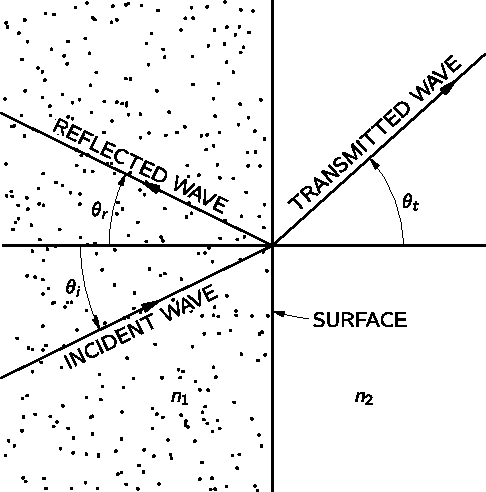
\includegraphics[width=0.7\linewidth]{fyz_fig0860.pdf}
      \caption{
               (\cite[s.~707]{Feynman02})}
      \label{fyz:fig0860}
    \end{figure}

    \begin{figure}[ht!] %\ref{fyz:fig0861}
      \centering
      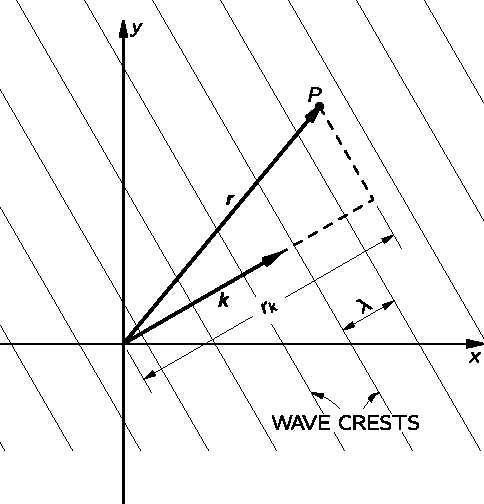
\includegraphics[width=0.7\linewidth]{fyz_fig0861.pdf}
      \caption{
               (\cite[s.~707]{Feynman02})}
      \label{fyz:fig0861}
    \end{figure}

    \begin{figure}[ht!] %\ref{fyz:fig0862}
      \centering
      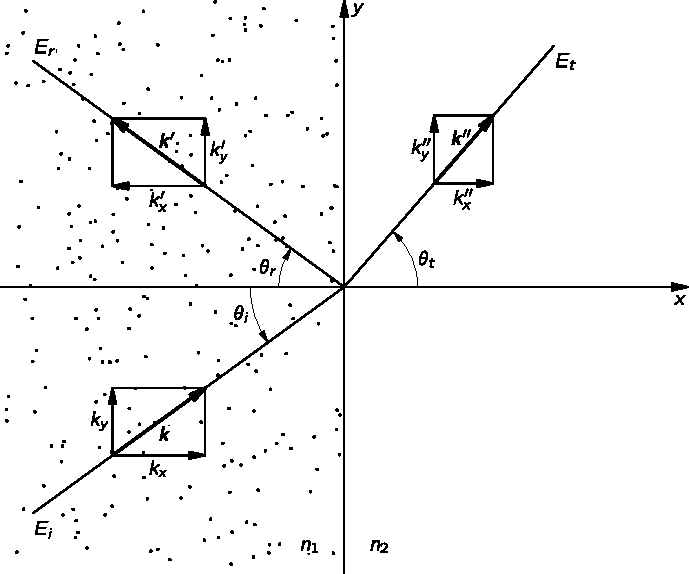
\includegraphics[width=0.7\linewidth]{fyz_fig0862.pdf}
      \caption{
               (\cite[s.~707]{Feynman02})}
      \label{fyz:fig0862}
    \end{figure}

    \begin{figure}[ht!] %\ref{fyz:fig0863}
      \centering
      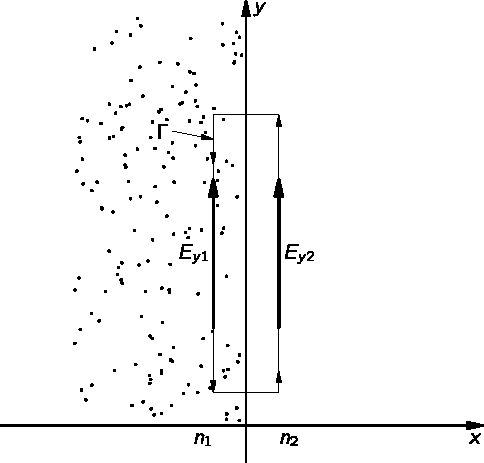
\includegraphics[width=0.7\linewidth]{fyz_fig0863.pdf}
      \caption{
               (\cite[s.~707]{Feynman02})}
      \label{fyz:fig0863}
    \end{figure}

    \begin{figure}[ht!] %\ref{fyz:fig0864}
      \centering
      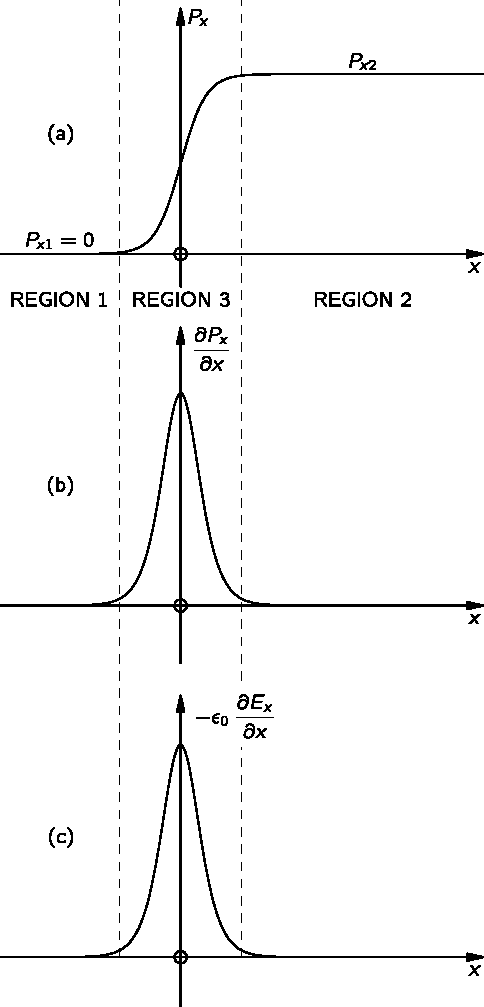
\includegraphics[width=0.7\linewidth]{fyz_fig0864.pdf}
      \caption{
               (\cite[s.~707]{Feynman02})}
      \label{fyz:fig0864}
    \end{figure}

    \begin{figure}[ht!] %\ref{fyz:fig0865}
      \centering
      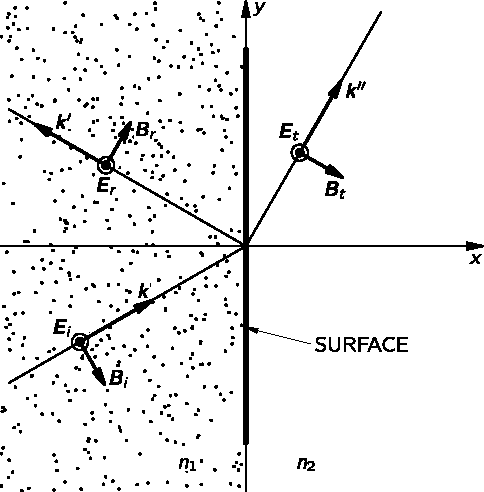
\includegraphics[width=0.7\linewidth]{fyz_fig0865.pdf}
      \caption{
               (\cite[s.~707]{Feynman02})}
      \label{fyz:fig0865}
    \end{figure}

    \begin{figure}[ht!] %\ref{fyz:fig0866}
      \centering
      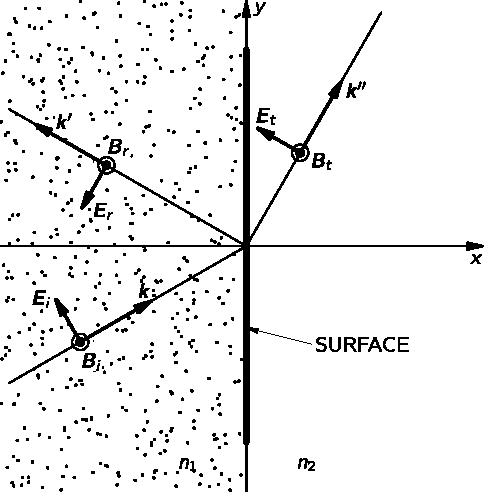
\includegraphics[width=0.7\linewidth]{fyz_fig0866.pdf}
      \caption{
               (\cite[s.~707]{Feynman02})}
      \label{fyz:fig0866}
    \end{figure}

    \begin{figure}[ht!] %\ref{fyz:fig0867}
      \centering
      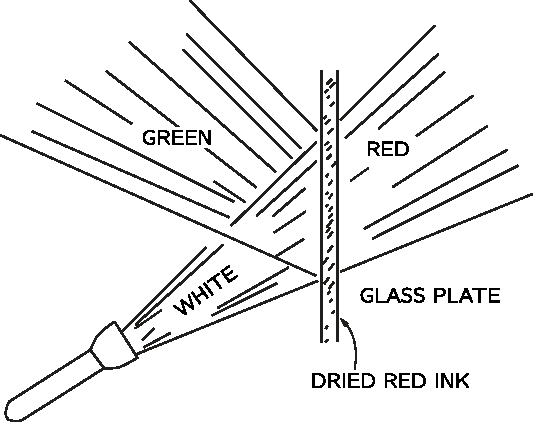
\includegraphics[width=0.7\linewidth]{fyz_fig0867.pdf}
      \caption{
               (\cite[s.~707]{Feynman02})}
      \label{fyz:fig0867}
    \end{figure}

    \begin{figure}[ht!] %\ref{fyz:fig0868}
      \centering
      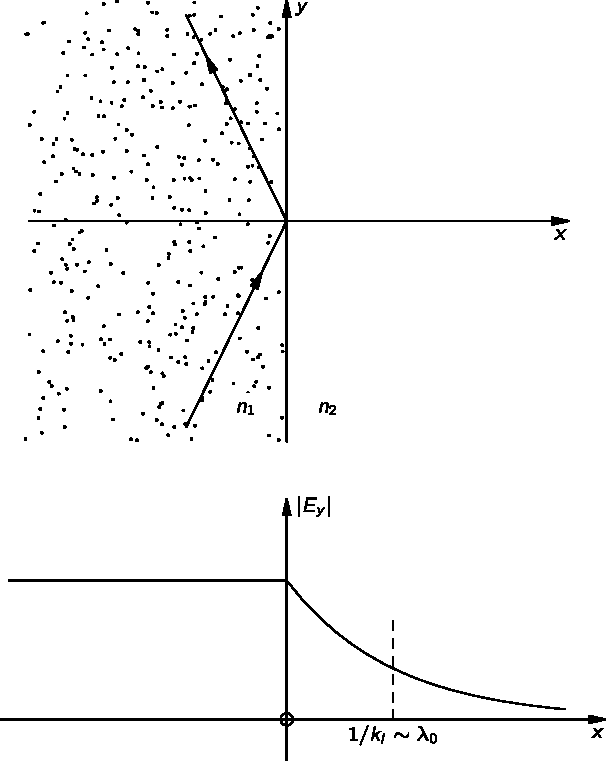
\includegraphics[width=0.7\linewidth]{fyz_fig0868.pdf}
      \caption{
               (\cite[s.~707]{Feynman02})}
      \label{fyz:fig0868}
    \end{figure}

    \begin{figure}[ht!] %\ref{fyz:fig0869}
      \centering
      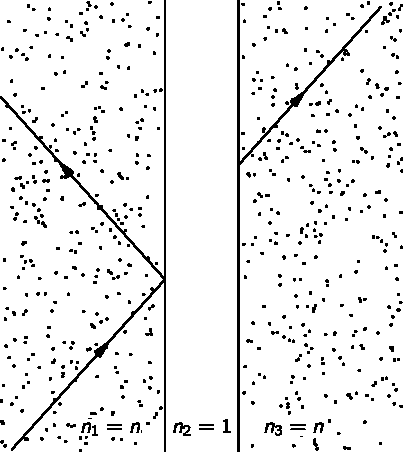
\includegraphics[width=0.7\linewidth]{fyz_fig0869.pdf}
      \caption{
               (\cite[s.~707]{Feynman02})}
      \label{fyz:fig0869}
    \end{figure}

    \begin{figure}[ht!]   %\ref{fyz:fig0870}
      \centering
      \subcaptionbox{\label{fyz:fig0870a}}{\luafigure[0.9]{fyz_fig0870a.pdf}}               \\
      \subcaptionbox{\label{fyz:fig0870b}}{\luafigure[0.9]{fyz_fig0870b.pdf}}               \\
      \subcaptionbox{\label{fyz:fig0870c}}{\luafigure[0.9]{fyz_fig0870c.pdf}}
      \caption{
               (\cite[s.~748]{Feynman02})}
      \label{fyz:fig0870}
    \end{figure}

    \todo[inline]{Kapitola fey2ch33 je nedodělaná, obsahuje pouze obrázky}
%} %tikzset
%---------------------------------------------------------------------------------------------------